\chapter{云计算基础软件架构介绍}
\label{chapter:techs}
本章我们将系统的介绍现有的云计算软件架构的两个核心部分:分布式存储和计
算模型。虽然在我们的研究过程中,这两者是紧密结合的,但是为了叙述方便,
在本章我们将他们分开描述。在这些分析和介绍中,我们将着重介绍和分析其跟
性能相关的部分,忽略安全性,易用性等在实际使用中更为关心的部分。在本章
最后一节,将从几个方面系统的分析现有系统存在的问题以及可能的解决方案。


\section{存储}
\subsection{GFS}
事实上,在2006年云计算概念被提出之前,云计算的基础软件架构就已经出现。其中影响最大的为Google与2004年后公开的Google File System和MapReduce两个分布式系统。在这两个系统的基础上,Yahoo!公司支持了Apache基金会下名为Hadoop的开源版本的研究和实现,并且逐渐构建了一套专用于大数据批处理的生态系统。

Apache Hadoop项目包含了包括HDFS(Hadoop Distributed File System),MapReduce计算框架,HBase半结构化数据库,Hive数据仓库等一系列分布式系统和工具。这其中以HDFS、MapReduce最为常用。HDFS是一种基于Google File System开发的分布式文件系统,因此在下文介绍中,除非特别点明两者的区别之外,我们简略的认为GFS和HDFS是等价的。

2003年,Google发表论文介绍了一个基于分布式块存储的文件系统,称为Google File System,该系统很好的支持了世界上最大规模的搜索引擎公司对数据存储的需求。GFS的基本架构如下图(\ref{fig:gfsarch})所示,由一个GFS master和若干个GFS Chunkserver组成。文件系统的层次结构和名字空间都存放在GFS Master节点中,客户端应用程序首先通过查询GFS master来获得欲访问的文件所在节点信息(chunk location),然后通过向特定的节点发送读写请求来完成数据传输过程。

\begin{figure}[]
\centering
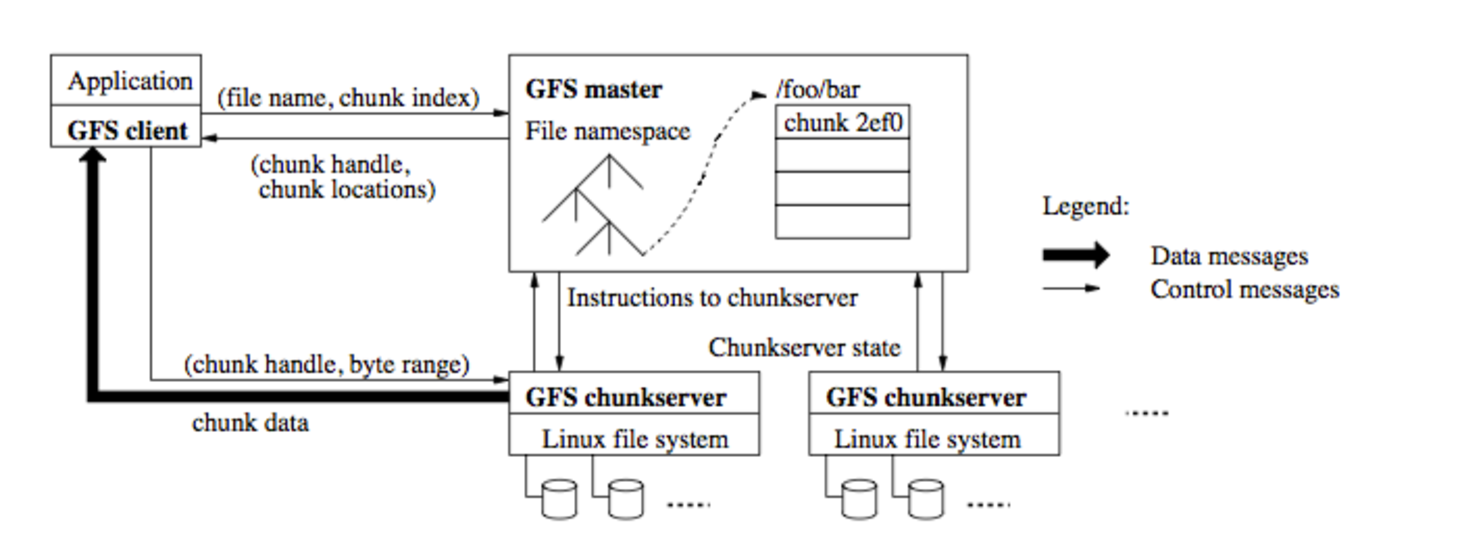
\includegraphics[width=6.5in]{../figures/gfsarch.pdf}
\caption{GFS文件系统的架构(摘自\textit{Ghemawat, S.; Gobioff, H.  Leung, S. The Google File System. ACM SIGOPS Operating Systems Review, 2003})}
\label{fig:gfsarch}
\end{figure}

Hadoop Distributed File System(HDFS)基本上按照GFS的架构来设计和实现,GFS master和chunkserver分别对应NameNode和DataNode。在HDFS上,任何一个文件都由预定义大小(默认64MB)的块组成,这些块被冗余存储于多个DataNode上(默认情况下,每一个块会存储在三个节点中)。由于HDFS多运行在由海量普通计算机构成的数据中心中,节点的失效和网络问题非常普遍,通过多备份数据极大的提高了系统的可用性和容错性。每一个DataNode需要和NameNode维持一个周期心跳用来检测节点是否失效以及网络是否可用,当NameNode发现某节点失效的时候会利用备份节点的数据来提供服务,并且尝试恢复失效节点,以维持每一个数据块三备份的状态。由于每一个客户端在访问HDFS中的数据时都需要向NameNode查询相关数据所在的DataNode位置信息,为了保证多个客户端程序读写的性能,HDFS的实现中会将所有的命名空间信息都存放在NameNode的内存中。

HDFS这种基于数据块的设计方法极大的提高了系统对于海量文件的存储能力。通过一个NameNode的管理,我们可以轻易的管理成千上万服务器构成的存储集群,提供PB量级的数据存储服务。然而,这里面却依旧存在很多问题,首当其冲的就是单NameNode节点的安全性问题。上面我们提到了,HDFS集群中任一个数据块都会存储在三个不同的DataNode节点中以保证某一个DataNode失效的时候仍然可以提供服务,然而如果NameNode节点失效,那么HDFS集群马上就不再能够提供服务了。为了解决这个问题,HDFS本身引入了SecondaryNameNode作为主NameNode的备份节点,它会不断的将数据存储的日志和HDFS的FSImage文件合并来维持一个当前状态的镜像文件。当主节点失效时, SecondaryNameNode会从现有的状态镜像文件中快速恢复出NameNode的状态并且提供服务。但是在实际使用中,由于集群规模较大,这一恢复过程可能超过十分钟,使得大规模集群整体离线的可能性依然较大。针对这一问题,2011年Borthakur et al.提出了使用AvatarNode代替NameNode和SecondaryNameNode的方案,系统架构如图(\ref{fig:avatar})所示.

\begin{figure}[]
\centering
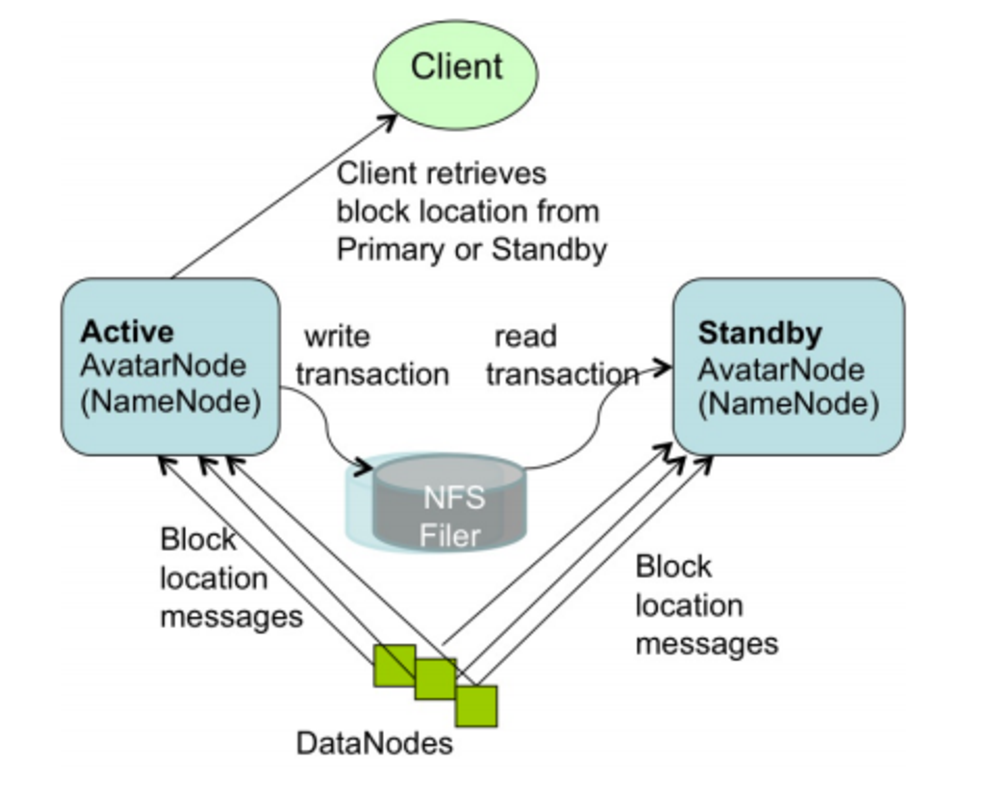
\includegraphics[height=4.25in]{../figures/avatarfb.pdf}
\caption{Avatar Node架构(摘自\textit{Borthakur, D et al. Apache Hadoop goes realtime at Facebook Proceedings of the 2011 international conference on Management of data, 2011})}
\label{fig:avatar}
\end{figure}

这样,一个HDFS集群就包含了两个avatar节点,active avatar和standby avatar。任一个avatar节点实际上都是一个正常的NameNode的包裹。HDFS文件系统镜像和日志都存放在NFS中,而不是本地。活动的avatar节点将所有的事务写入在NFS中的log文件中,与此同时,standby avatar节点将从NFS中打开相同的log文件,读入并且不断的将新写入的事务应用到本地存储的命名空间中,从而使得本地的命名空间和当前活跃avatar节点上的命名空间保持尽量一致。所有的DataNode不仅仅和active avatar节点交流还会和standby avatar节点交流,这样就使得standby的avatar节点时刻保持着最新的块位置信息,以保证在活跃节点失效的时候,standby节点能够在一分钟内开始提供服务。

另外一个HDFS系统暴露的重要问题就是存储容量瓶颈。通过对HDFS架构的介绍我们可以发现,虽然HDFS的存储容量似乎仅仅是由DataNode的数量和容量决定的,通过不断增加DataNode的数目似乎可以极大的提高存储能力。然而实际上,真正的瓶颈还是在NameNode上。为了保证客户端读取速度,我们必须把存储的命名空间信息存储在NameNode的内存中,随着存储数据量的扩展,NameNode的内存容量逐渐成为了系统瓶颈。Konstantin V. Shavachko发表论文详细探讨了HDFS文件系统的瓶颈。通过对当时最大的HDFS集群(运行在Yahoo!)的实际运行数据的搜集和分析,给出了单个NameNode服务器上内存容量和整个HDFS集群存储容量上限的关系:每一个块的位置信息都需要在NameNode中占据超过200个字节的内存,而在一个文件平均包括1.5个块的集群中,每一个文件就大概需要600个字节的内存空间。这样,如果要存储超过1亿个文件,那么NameNode至少就要有60GB的内存。如果该HDFS集群中每一个块为128MB,并且备份三分,那么总的存储空间就是60PB(NameNode需要60GB内存)。通过对Yahoo!公司内部运行的最大HDFS集群(4,000个节点,存储14PB的文件)的数据进行分析,如果部署一个1万台服务器的HDFS集群,并且仅仅有一个NameNode,那么它能够为超过1百万个读客户端提供服务,然而面对1万个写客户端就会崩溃。这也就意味着HDFS的架构不具备线性扩展性。1万台服务器的扩展度貌似很高,然而实际上现在在一个数据中心中超过万台服务器已经是非常正常的情况了,再加上大量的小文件存储也会使得块利用率降低,给NameNode产生更大的压力,因此就连HDFS的开发团体也提出了一个针对NameNode内存大小优化的建议(HADOOP-168, “NameNode Memory Size Estimates and Optimization Proposal”)。

解决该问题最好的办法就是引入分布式的NameNode。M.K. McKusick et al.提出了一种新的GFS Namespace 服务器的架构。这种新的架构包含了数以百计的Namespace服务器,每一个服务器上最多支持超过1亿个文件。由于NameNode容量的提高,每一个文件可以被划分为更加细粒度的块(由64MB可以减少到1MB),用以支持小数据存储。HDFS-dhh就是该思想的一个具体实现,在该实现中,它使用了HBase来代替HDFS中的单NameNode,试验结果表明改进后的HDFS集群的写性能可以做到线性扩展,极大的提高了HDFS的应用范围。

这里我们主要描述了HDFS的两个缺陷,单点故障和存储容量上限。这两个缺陷实际上都是由于HDFS中为了设计简单而引入的单NameNode结构引起的。这两个缺陷随着云计算技术的不断发展,没有渐渐显示反而越来越严重。特别是由于越来越多的数据种类开始需要在分布式存储环境下进行存取,比如小的键值数据,实时更新的数据流等,HDFS这种面向块的海量存储方案显得过于简单和低效,这种矛盾也不断催生着新的技术。其中比较典型的包括Dynamo、HBase、Redis,RamCloud等。

\subsection{Dynamo}

Dynamo是2006年由Amazon公司设计实现的一种高可用的键值存储系统,它被设计成为完全不同于GFS类型的新型存储系统:
\begin{itemize}
\item 从存储内容来说,Dynamo是一种存储键值对的存储系统。这也意味着它需要提供更好的随机读写的能力;需要提供更好的数据空间管理能力;需要更细粒度的容错能力;
\item 从应用场景来说,Dynamo主要应用于Amazon特有的‘永远可写’的场景中。比如在Amazon网站的购物车应用中,我们永远希望用户任意一次的“加入购物车”行为都能够成功,不管这次请求写入的节点是否失效或者数据中心网络是否出现了分离错误。而HDFS这种GFS类型的存储系统面对的往往是需要海量离线存储能力的场景。
\item 从架构上来说,Dynamo彻底抛弃了GFS的单中心节点架构,转而提出了一套完全没有中心节点的P2P架构:所有的节点都等价的提供服务,节点和节点之间松耦合:单个节点失效不会影响到别的节点。
\end{itemize}

为了满足Amazon这样的世界上最大的电子商务公司对底层基础架构的可靠性和伸缩性的需要,Dynamo综合了一些著名的技术来实现工业级的可伸缩性和近乎苛刻的可用性。
\begin{itemize}
\item 采用动态哈希表和一致性哈希来进行数据划分和复制备份;
\item 使用多版本和矢量时钟技术来提供一致性;
\item 多副本之间的一致性由仲裁算法来保持一致性;
\item 采用反熵(anti-entropy based recovery)的恢复策略;
\item 采用基于gossip的分布式故障检测及token协议。
\end{itemize}
正如Amazon的CTO在SOSP 2007会议上提到的那样\textit{“据我所知Dynamo是最早的综合使用所有这些技术的生产系统,并且通过这样做也得到了不少教训.”}。由于这些技术在大规模分布式系统中的重要地位,以及它对于我们提出的存储系统中技术的启发作用。我们将分开介绍它们,并且对于每一个技术要点都结合Dynamo中的实际设计进行分析。

\subsubsection{数据分割和一致性哈希}
数据分割是指将数据空间按照某种规则分别存储到分布式集群中的某一台机器的行为,它也是所有分布式存储系统首先要解决的问题。GFS类的系统的数据分割是非常自由的,系统可以为某一块数据任意指定所存储的节点,然而这种自由带来的问题就是系统必须具备主节点,并且在主节点上要显式的记住所有节点的位置信息,以便之后读写的时候能够找到数据的位置信息。

与这种主从结构对应的就是完全对等的分布式存储架构。为了在这种架构上进行数据局分割,人们引入了分布式哈希的概念以及一致性哈希的实现。分布式哈希(distributed hash table)是指一类去中心化的分布式系统,该系统能够提供类似哈希表的查询功能。分布式哈希表中同样存放键值对,其中任意一台服务器必须能够有效的根据给定key能够查询到对应value的值。key到valaue的映射信息应该是由所有节点共同维护的,并且使得其中一些节点失效也不会对整个映射信息产生巨大的变化。该特点就能够允许分布式哈希系统能够在非常大量的节点上扩放,并且支持节点随时加入、退出以及失效。分布式哈希所指的为一类具备上述特征的系统,而具体如何实现这类系统并没有给出完整的解答,而一致性哈希则正是能够实现分布式哈希的一类方法。它有很多变种和具体的实现,这些实现比较核心的区别包括两点:1)如何划分key空间;2)如何路由查询。首先我们结合Chord这个比较经典的一致性哈希实现来介绍其基本概念,之后将详细介绍Dynamo是如何实现自己的一致性哈希算法的。

首先定义一个函数$\delta(k_1, k_2)$,定义了两个键$k_1$和$k_2$的距离。于此同时定义集群中任意一台服务器的都有一个id,且该id所取的值空间和$k_i$的值空间相同。那么节点$ID=i_x$就应该负责存储所有距离$i_x$最近的所有的$k_m$。在Chord中,所有的key都被看做一个环上的点,而$\delta(k_1, k_2)$就定义为沿着环顺时针方向的距离。这样,一个key空间就被划分为多个连续的环上的段,而段与段的交界点就是节点id。若$i_1$和$i_2$是两个连续的节点,那么节点$i_2$就应该存储所有落在$i_1$和$i_2$之间的key。

由于分布式哈希系统要求所有节点都是同等地位的,因此每一个节点都要保持一个到它的”邻居节点”的链接,这些虚拟的“链接”构成了在真实网络之上的Overlay网络,Overlay网络的结构也成为Overlay拓扑,它决定了分布式哈希的结构。所有有效的拓扑都必须具备一下性质:对于任何一个key,任意一个节点要么存储了该key的信息,要么能够提供一个链接指向一个距离该key更近的节点。Chord中,每一个节点会储存一个路由表,表内按顺时针按照离本节点2、4、8、16...的距离选定$\log2N$个其他节点的ip信息来记录。当需要查询的时候,某节点首先从自己的路由表中找到一个和数据key距离最近、并且存活在网络中的节点\textit{next}。如果恰好该key应由该节点负责存储,那么结束,否则由\textit{next}节点进行递归查找。

由于对性能的要求远比广域网上的P2P软件苛刻,Dynamo的分布式哈希实现中摒弃了多跳路由,转而使用单跳路由。这也意味着每一次查找键所在节点信息都只需要一次查询即可。为了实现这一点,Dynamo的一致性哈希在现有哈希算法的基础上引入了虚节点的概念,每一个虚节点对应的就是上面我们所介绍的节点,而真正的服务器却是和虚节点对应的,一个实际物理节点可能需要存储多个虚节点的数据(称为token)。整个Hash空间被平均分为$Q$份,$Q$满足下面条件:$Q\gg N$以及$Q \gg S*T$,$S$表示系统中节点的数量。每一个物理节点都会被指派给$Q/S$个token。当一个节点离开系统的时候,它的所有token会被随机的分布到剩余的节点上,以保持每一个物理节点有$Q/S$个token的属性。该算法跟传统算法相比,具备更好的负载均衡特性,并且能够提供更高的存储效率,Dynamo的一致性哈希算法的示意图如图(ref{fig:dynamo})所示。

\begin{figure}[]
\centering
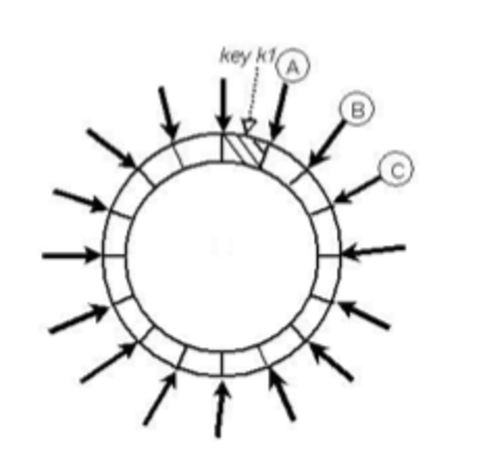
\includegraphics[height=2.25in]{../figures/dhtdynamo.pdf}
\caption{Dynamo采用的一致性哈希算法示意图。A、B、C为三个不同的节点,它们都负责存储key k1.黑色箭头指明了不同节点的token位置。(摘自\textit{DeCandia, G.; et al. Dynamo: Amazon's highly available key-value store. ACM SIGOPS Operating Systems Review, 200})}
\label{fig:dynamo}
\end{figure}

\subsubsection{CAP和最终一致性}

CAP定理(图\ref{fig:cap})是分布式计算中一个非常基础的定理,它定义了一个分布式系统的三个希望获得的特性:一致性(Consistency),可用性(Availability),以及分割容忍(Partition tolerance),并通过理论分析证明这三个特性不可能同时存在于一个分布式系统中。

\begin{figure}[]
\centering
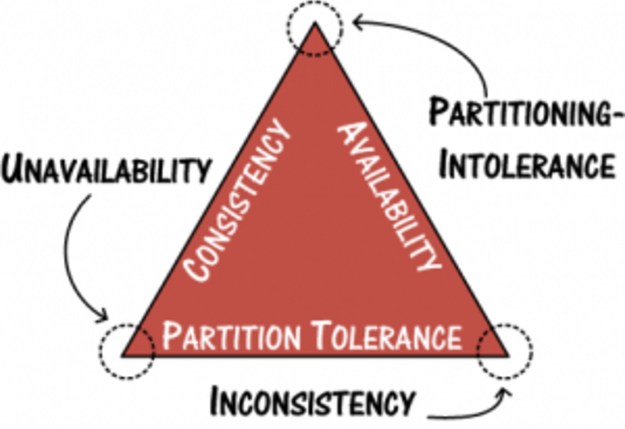
\includegraphics[height=2.25in]{../figures/cap.pdf}
\caption{CAP定理示意图(摘自\textit{互联网})}
\label{fig:cap}
\end{figure}

CAP定理直接为分布式系统定义了一个极限,所有的系统都要在这三个希望具备的特性中做出取舍。比如分布式数据库需要支持ACID语义,那么就只能放弃分割容忍的能力;而Dynamo这种运行在多个数据中心中,必须能够”永远”在线的云计算基础软件却不能放弃分割容忍以及可用性的特质,因此只能放松系统对一致性的要求,从而产生了弱一致性的系统。

假设存在三个独立的客户端进程A,B,C,他们都需要访问一个位于云端的分布式存储系统。A进程首先写入一个值,之后B和C进程会读取该值。如果B和C都一定会读取到A写入的值,我们可以称这个存储系统是一个强一致的存储系统;而如果B和C不一定会读到最新的值,那么我们称其为弱一致的存储系统。从A更新该数据到另外一个独立进程读取到更新后的数据的时间差成为不一致窗口(inconsistent window)。最终一致性就是弱一致性系统的一种特定的形式:存储系统保证如果某数据没有新的修改,那么最终所有对该数据的读取都将返回最新的值。其实这种系统早就已经出现了,比如DNS(Domain Name System),比如传统关系数据库中的异步主备份,都是满足最终一致性的系统。

Dynamo提供最终一致性,更新操作异步的传播到所有副本,这样即便在网络分割的场景下,Dynamo客户端无论当前连接在哪一个分片中,都能够写入。为了提供这种保证,Dynamo将每次数据修改的结果当做一个新的且不可以改变的数据版本,它允许系统中同时出现多个版本,这些版本信息将反映给开发者,而由开发者来协调这些可能冲突的版本。为了尽量减少冲突版本的数量,Dynamo还引入了矢量时钟来捕捉不同版本对象的因果关系。矢量时钟是一个由(nodeId, counter)组成的对,如果一个时钟对象上的计数器在第二个时钟对象上小于或等于其他所有节点的计数器,那么第一个是第二个的祖先,可以被忽略,否则这两个变化被认为是冲突,并要求协调。

为了保持多副本的一致性,Dynamo使用基于仲裁(quorum)的一致性协议。该协议有两个关键值:$R$和$W$. $R$是一个成功的读取操作的最少参与节点数。$W$是必须一个成功的写操作的最少参加节点数。设定$R$和$W$,使得$R+W>N$时将产生一个强一致的副本模型。在此模型中,一个读写操作延时是由最慢的读或写的副本决定的。因此从性能的角度考虑,Dynamo中$R$和$W$通常配置为小于$N$,为客户提供更好的性能。

当收到写请求时,协调节点生成新版本向量时钟并在本地写入新版本,然后将新版本(与新的向量时钟一起)发送给首选列表中的排名前N个的可达节点。如果至少W-1个节点返回了响应,那么这个写操作被认为是成功的。同样,对于一个读请求,协调节点从首选列表中排名前N个可达节点处请求所有现有版本的数据,然后等待R个响应, 然后返回结果给客户端。如果最终协调员收集的数据的多个版本,它返回所有它认为没有因果关系的版本。不同版本将被协调,并且取代当前的版本,最后写回。

%\subsubsection{Gossip协议以及成员检测}
%分布式系统中需要持续的进行成员检测以保持对系统状态的 @TODO: 添加该部分
\subsubsection{Cassandra}
  Cassandra是由Facebook的工程师实现的一个分布式的存储系统,其设计目标即为在大量的普通PC的基础之上,能够存储海量的数据,同时提供无单点故障的、高可用的服务质量。Cassandra可以看作是Bigtable和Dynamo的结合品:首先,Cassandra的数据模型与Bigtable非常类似,都是将结构化以及半结构化的数据存放在数据表中;其次,都使用了Dynamo那种去中心化、松散的架构。考虑到Cassandra是由一批来自Amazon的Dynamo项目组的工程师开发的,就不足为奇了。Cassandra同样使用分布式一致性Hash来分割数据,不同的是将实际的节点和虚拟结点映射的方法不同。多备份算法基于ZooKeeper实现,而非Gossip协议。而机群中成员信息的维护和管理都是基于一种anti-entropy的Gossip算法。Cassandra中的数据都是通过本地文件系统进行持久化的,一个典型的写操作将首先写入log文件,其次写入内存中的数据结构。通过这种方式保证所有的更新操作都被持久化到本地,而所有的读都是直接从内存中读取的,因此Cassandra的读效率非常高。


\subsection{Megastore}
Megastore是由Google于2011年公开的一种存储系统,它整合了当时流行的NoSQL数据库的扩放行,于此同时也提供了传统RDBMS具备的易用性(比如SQL查询支持,ACID语义支持)。它提供了强一致性保证、高可用性,并且在细粒度的数据分片中提供了ACID的语义,这听起来似乎和之前提到的CAP定理有矛盾,事实上Megastore是通过给应用程序细粒度的管理数据分片和本地性的能力来避免CAP的限制:在Megastore中以EntityGroup作为基本的独立数据集合,一个EntityGroup中的数据并且会在不同的数据中心间同步复制。除此之外,Megastore还使用Paxos协议避免了之前所提到的分布式主节点需要将写前日志(write-ahead-log)复制到多个节点的耗时操作。

\begin{figure}[]
\centering
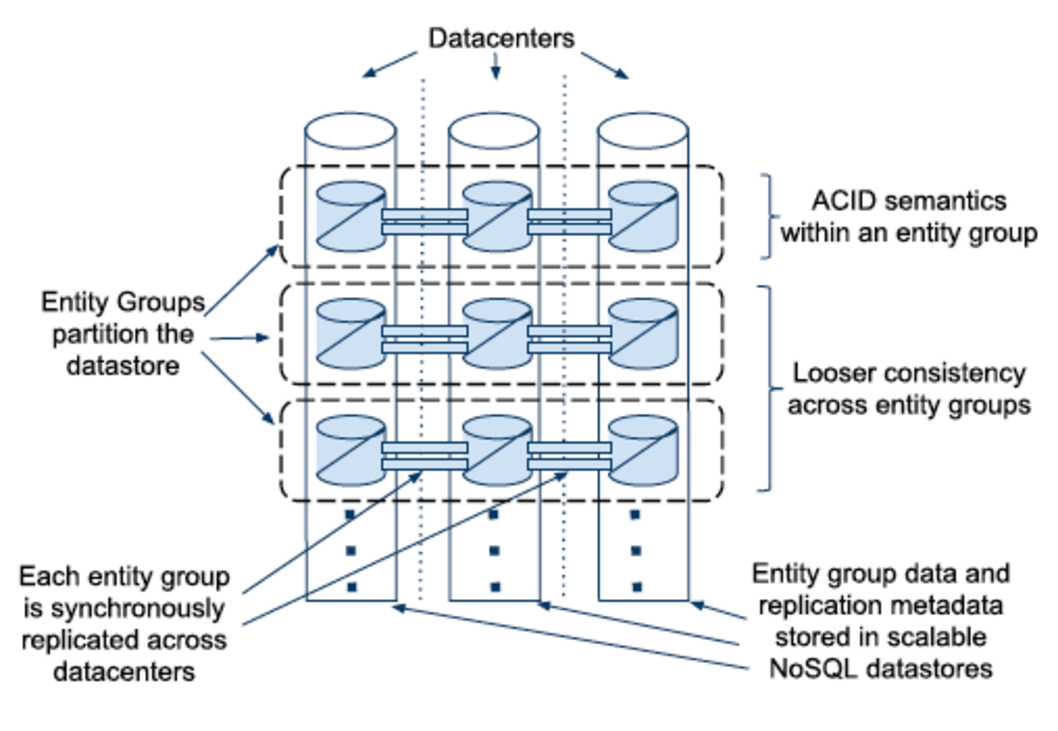
\includegraphics[width=5in]{../figures/megastore.pdf}
\caption{Megastore架构图(摘自\textit{Baker, J. et al. Megastore: Providing scalable, highly available storage for interactive services. Proc. of CIDR, 2011})}
\label{fig:megastore}
\end{figure}

图(\ref{fig:megastore})展示了EntityGroup的结构以及它们是如何在不同的数据中心之间进行复制的。在一个EntityGroup内部的所有操作都依赖于Paxos算法来确保其ACID的语义,而跨EntityGroup的操作则依赖于比较笨重的两阶段提交协议,或者使用异步消息的最终一致方案。在一个数据中心内部,Megastore使用Bigtable来做基础的容错存储。Megastore的创新点主要体现在下面几个方面:1)设计了EntityGroup方案给用户提供了足够的一致性的灵活性;2)使用Paxos算法来保证EntityGroup内部数据的强一致性。3)基于已存的系统:Bigtable和GFS并且和SQL模型相结合。尽管Megastore在Google内部已经开始大规模使用,然而在Google之外却没有引起太多的关注,核心原因应在于Megastore引入了过多的不是很成熟的优化,使得该架构更像是一个专用存储系统。

\subsection{RamCloud}

近期,随着基于云的应用程序的不断发布和流行,特别是基于社交网络的各种服务,交互式在线服务,人们开始注意到基于磁盘的传统存储系统相对于这些在线服务,问题也越来越大,尤其在速度上非常明显。另一方面,新的存储介质的发展也非常迅速,包括非易失性内存(PCM, Memristor以及STTRAM)等变得越来越便宜。因此基于这些新的存储介质来构建新型的分布式文件系统的想法也越来越多,其中非常重要的一个工作便是基于内存(易失的动态内存)的分布式存储系统RamCloud。Stanford大学的一个研究小组在2009年提出将所有的数据都存放在DRAM中从而构建一个大规模的、可扩放的存储系统。

一个RamCloud机群包含了成千上万的现成的服务器,每一个都包含性价比最高的内存容量(24-64GB),而RamCloud将这些内存聚合成一个存储系统,它将备份数据放置在磁盘以及Flash上以使其持久及可用。下图展示了一个典型的RamCloud机群的结构。它包含了大量的存储服务器,每一台存储服务器包含两个部分:1)主服务,其负责在内存中管理RAMCloud对象,并且负责处理客户端的请求;2)备份服务,其存储了来自别的主节点的备份数据,并且将其存放到磁盘和Flash中。

\begin{figure}[]
\centering
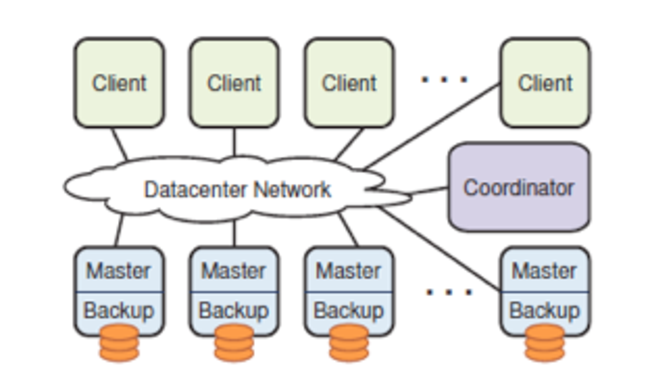
\includegraphics[width=4.5in]{../figures/ramcloud.pdf}
\caption{RamCloud架构图(摘自\textit{Ousterhout, J. et al. The case for RAMClouds: scalable high-performance storage entirely in DRAM. ACM SIGOPS Operating Systems Review, ACM, 2010})}
\label{fig:ramcloud}
\end{figure}


每一个RAMCloud实例都会包括一个单独的服务器,成为协作者(Coordinator)。其负责管理配置信息,比如存储服务器的网络地址,以及对象的位置信息。协作者将对象放置到不同的存储服务器以:一个连续的key域存储在一个表中。较小的表会存放在一个存储节点中,较大的表会被分割并且存储与多个节点。 客户端程序不会控制表的配置,而写作者会存放表和存储服务器之间的映射信息。RAMCloud客户端库将会保存一些缓存信息以防多次访问协作者。

  基于内存的存储系统面临的一个大问题就是如何保证在内存掉电并且丢失所有数据的情况下,保证数据的可用性。一种简单的做法就是将每一个对象复制到多个存储服务器的内存中,在RAMCloud中,作者认为这并不是一个好做法,因为这将导致三倍的内存消耗。因此在RAMCloud只在内存中保留一份数据,而多个拷贝则被存放在别的存储服务器的磁盘中,存储在磁盘时,将使用日志形式,以保证I/O效率。

\begin{figure}[]
\centering
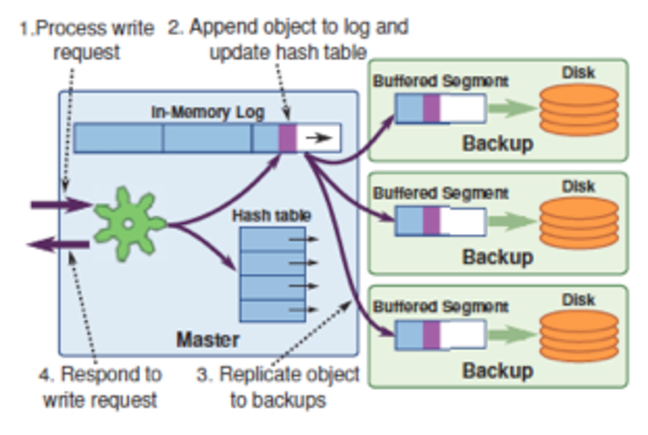
\includegraphics[width=4.5in]{../figures/ramcloudlog.pdf}
\caption{RamCloud Log访问的结构图(摘自\textit{
Ongaro, D.; et al. Fast crash recovery in RAMCloud. Proceedings of the Twenty-Third ACM Symposium on Operating Systems Principles, 2011})}
\label{fig:ramcloudlog}
\end{figure}

如上图所示,当一个存储节点中的主服务收到一个写请求的时候,它将首先更新自己内存中的Hash表,并且将新的数据转发到多个备份节点中,它们将把这些新数据缓存在它们的内存中,而最终被写到本地磁盘中。备份节点必须使用备份电源来确保即便在断点时,缓存中的数据也能被写入到本地磁盘中。
  由于我们在别的节点的磁盘中备份数据,从而导致若当前节点失效,那么数据需要重新从磁盘中读入,并且建立新的映射关系,这个时间会非常漫长。以当前典型的磁盘I/O效率,一个64GB的内存镜像如果单机恢复,至少需要几分钟的时间。为了达到1~2秒内恢复数据的要求,RAMCloud实现了一种分布式的数据恢复策略。


\begin{figure}[]
\centering
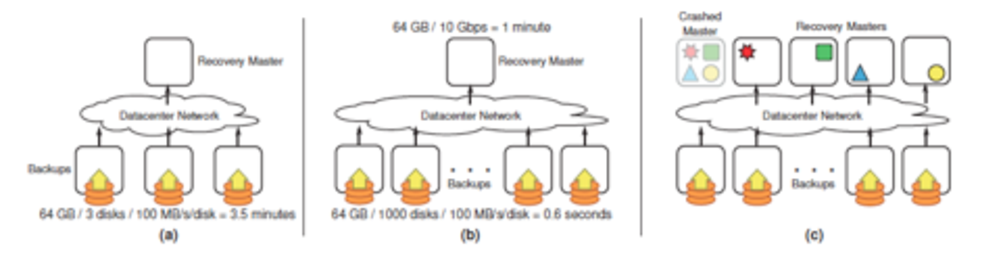
\includegraphics[width=4.5in]{../figures/ramdist.pdf}
\caption{RamCloud 多备份结构(摘自\textit{
Ongaro, D.; et al. Fast crash recovery in RAMCloud. Proceedings of the Twenty-Third ACM Symposium on Operating Systems Principles, 2011})}
\label{fig:ramdist}
\end{figure}

如上图所示,(a)图展示了如果每一个主服务的数据都被镜像到少数的几台机器的情况下,恢复64GB的数据所需要的时间,可以看出瓶颈在于本地磁盘的IO速度;b)图则展示了,将日志文件备份到很多台服务器上,可以避免本地磁盘IO瓶颈,然而将这些日志文件传输到欲恢复的服务器之上,则需要较长的时间来进行重新生成内存映像,从而导致瓶颈;c)图则展示了将日志文件存放在多个服务器上,并且在多个服务器上同时进行恢复操作的情况,能够极大的提高效率。RAMCloud基于C图展示的原理实现了快速的错误恢复,兵以实验证明可以在秒级时间内恢复60GB左右的数据。

  RAMCloud的设计思路和目标以及遇到的一些问题都非常具有启发性。由于内存在随机访问上的优势,能够极大的降低系统的访问延时,提高吞吐量,非常适应与移动云计算环境对存储系统的要求。因此未来将大量的活跃数据放置于内存之上是非常有必要的。虽然前面提到的Cassandra和Bigtable等系统都很大程度上利用了内存的高速特性,但都是作为缓存来用的,这与RAMCloud中所提出的将内存完整的视作存储介质不同。RAMCloud不仅需要考虑读,更要考虑写。比如在写效率同样高于磁盘百倍的前提下,完成数据的可用性和持久性的设计。这也是基于内存的存储系统的关键。


\section{计算模型}
\subsection{MapReduce及其问题}
MapReduce自从2006年由Google提出,并且之后由Apache基金会以Hadoop项目开源实现,当前已经成为云计算平台中的标准配置。全世界数以千计的数据中心时刻运行着百万个MapReduce任务。作为一个批处理的计算模型,MapReduce非常适合于进行日志分析、离线推荐、或者单轮的PageRank算法。然而MapReduce依旧存在很多的问题:
\begin{itemize}
\item 不能很好的支持小的任务或者交互式任务。来自Google内部的经验,一个MapReduce任务平均需要8分钟的时间来执行,而一个PageRank算法重新运行一轮甚至需要几天的时间。这导致现有的MapReduce十分不适合一下几种任务:实时搜索、在线推荐或者广告系统。比如,在线推荐系统中,我们需要根据当前用户点击和浏览数据来计算新的推荐数据,这应该在几秒内实现,所以很明显的,现有的MapReduce是不符合的。
\item 不适合迭代式的数据处理。许多数据分析技术都需要交互式计算,包括新型的PageRank算法,HITS(Hypertext-Induced Topic Search),递归关系查询,神经网络分析,社交网络分析等。这些技术都有一个共同的特点:数据都是被迭代处理,直到计算收敛或者到达停止条件。MapReduce不能很好的支持这种迭代式的数据分析程序,开发人员只能通过编写驱动程序来手动的启动和管理多轮MapReduce工作。而这种开发方式显然不是一个好方法,1),每一轮迭代中,数据必须不断的重新载入,重新处理,这将极大的浪费I/O,网络带宽和CPU资源;2),停止条件或者收敛判断往往还需要一个额外的MapReduce来进行判断,这将引入非常大的延迟。
\item	MapReduce不适合进行数据源不断增加的分析任务。许多数据分析技术都需要对数据集进行递归计算,比如实时搜索引擎中所使用的PageRank算法。当爬虫爬取到部分新增网页,如果运行一个完整的MapReduce则极大的浪费了计算资源。
\item 使用MapReduce的编程框架,应用程序不能在线访问计算的任何中间状态,只能通过将不同的数据流进行聚合来模拟传统的共享内存结构,这也是许多迭代程序和递增程序所需要的。
\end{itemize}

  为了解决这些问题,许多都在进行中,去改进或者尝试重新设计数据处理模型。下面我们将依次介绍其中一些典型代表,并且最后帮助引出我们所提出的移动云计算平台中的数据处理平台。

\subsection{迭代处理模型}
HaLoop is a modified version of the Hadoop MapReduce framework that is designed to serve the iterative programs. The authors stated that HaLoop not only extends MapReduce with programming support for iterative applications, it also dramatically improves efficiency by making the task scheduler loop-aware and by adding various caching mechanisms.

HaLoop extends MapReduce and is based on two simple intuitions. First, a MapReduce cluster can cache the invariant data in the first iteration, and then reuse them in later iterations. Second, a MapReduce cluster can cache reducer outputs, which makes checking for a fix-point more efficient.

\begin{figure}[]
\centering
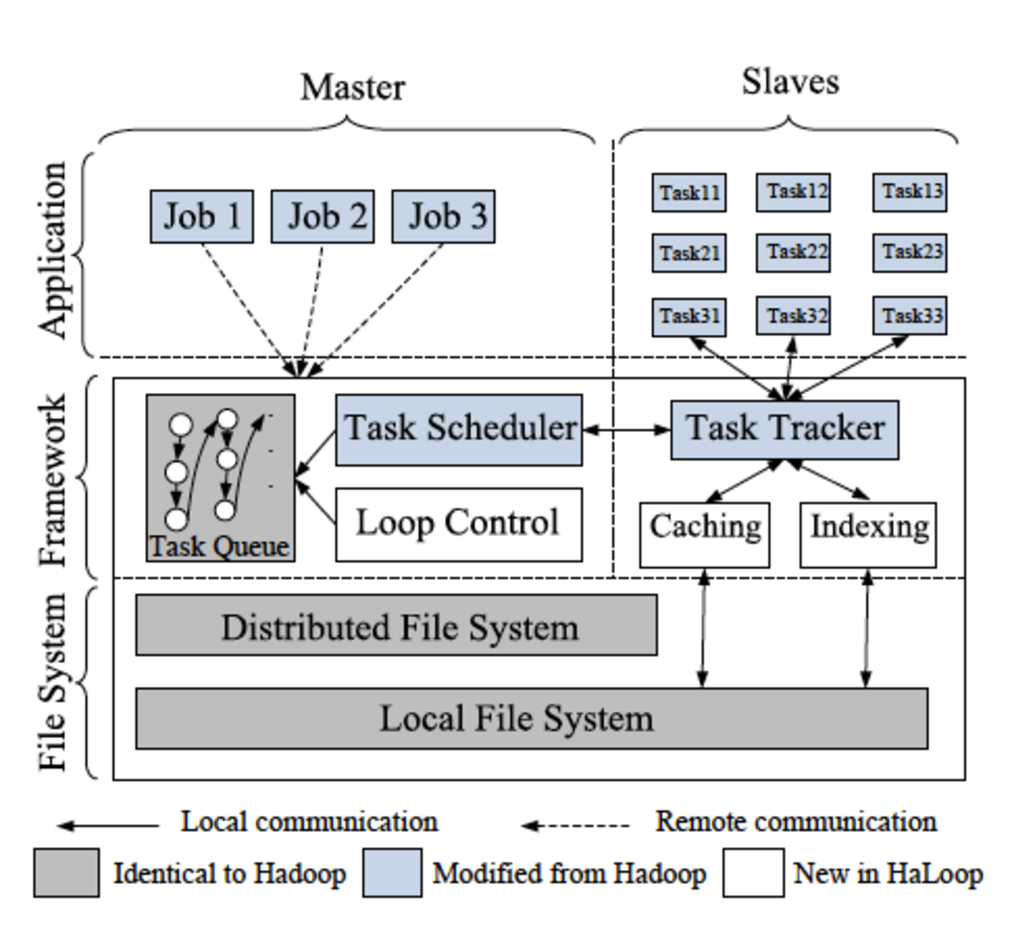
\includegraphics[width=5in]{../figures/haloop.pdf}
\caption{Haloop架构图(摘自\textit{Bu, Y. et al. HaLoop: Efficient iterative data processing on large clusters. Proceedings of the VLDB Endowment, VLDB Endowment, 2010})}
\label{fig:haloop}
\end{figure}

Fig.\ref{fig:haloop} illustrates the architecture of HaLoop. The system is divided into two parts: one master node and many slave nodes. A client submits jobs to the master node. For each submitted job, the master node schedules a number of parallel tasks to run on slave nodes. There are several changes to the basic Hadoop MapReduce framework. First, HaLoop's master node contains a new loop control module that repeatedly starts new map-reduce steps that compose the loop body, until a user-specified stopping condition is met. Second, HaLoop uses a new task scheduler for iterative applications that leverages data locality. Third, HaLoop caches and indexes application data on slave nodes.

The iterative programs that HaLoop supports can be distilled into the following core construct:
\begin{equation}
R_{i+1}=R_0 \cup (R_i \bowtie L)
\end{equation}
Where R0 is the initial result and L is an invariant relation.

To write a HaLoop program, a programmer specifies the loop body and optionally the specifies a termination condition and loop-invariant data.  HaLoop defaults to testing for equality from one iteration to the next to determine when to terminate the computation. To specify an approximate fix-point termination condition, the programmer uses the following functions: SetFixedPointThreashold, ResultDistance, SetMaxNumOfIterations...

HaLoop has a loop-aware task scheduler. It can take advantage of inter-iteration locality: that task (either mapper or reducer) that processes a specific data partition D is scheduled on the pysical node where D was processed in last iteration. HaLoop'
s scheduler keeps track of the data partitions processed by each map and reduce task on each physical machine, and it uses that information to schedule subsequent tasks inter-iteration locality into account. Besides, HaLoop aslo caches the data partitions on the physical node's local disk for subsequent re-use, to further accelerate processing. It is automatically re-loaded, either from map task physical nodes, or from HDFS. Accroding the experiments, the loop-aware scheduler and the cache mechanism help HaLoop archieve much better performance than Hadoop for iterative applications.

\subsubsection{Twister}
Twister is an enhanced MapReduce runtime that supports iterative MapReduce computation. It uses a publish/subscribe messaging infrastructure for communication and data transfers, and supports long running map/reduce tasks, which can be used in "configure once and use many times" approach. In addition, it provides programming extension to MapReduce with "broadcast" and "scatter" type data transfers.

\begin{figure}[]
\centering
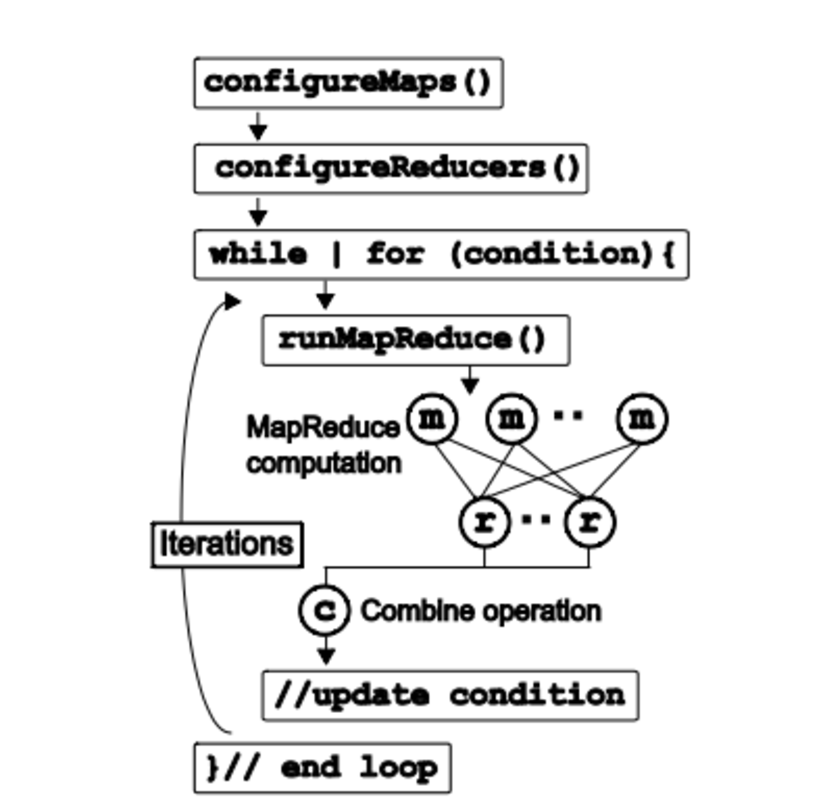
\includegraphics[width=3.5in]{../figures/twister.pdf}
\caption{Iterative MapReduce programming model supported by Twister(摘自\textit{Ekanayake, J.; et al. Twister: a runtime for iterative mapreduce. Proceedings of the 19th ACM International Symposium on High Performance Distributed Computing, 2010})}
\label{fig:twister}
\end{figure}

Fig.\ref{fig:twister} shows the extended programming model in Twister. To support map/reduce tasks operating with Static data and Dynamic data, Twister introduced a "configure" phase for map and reduce tasks, which can be used to load any static data at the map and reduce tasks. Twister proposes long-running map/reduce tasks similar to the parallel processes in many MPI applications that last throughtout the life of the computation. The long running map/reduce tasks will load static data in distributed memory to reduce the reloading time in each iteration.

Twister is a distributed in-memory MapReduce runtime optimized for iterative MapReduce computations. It reads data from local disk of the worker nodes and handles the intermediate data in distributed memory of the worker nodes. Fig.\ref{fig:twisterarch} shows the archtecture of the Twister runtime, which comprises of three main entities: 1) client side driver that drives entire MapReduce computation, 2) Twister Daemon running on every worker node, 3) the broker network. During the initialization of the runtime, Twister starts a daemon process in each  worker node, which then establishes a connection with the broker network to receive commands and data. The daemon is  responsible for managing map/reduce tasks assigned to it, maintaining a worker pool to execute map and reduce tasks, notifying status, and finally responding to control  events. The client side driver provides the programming API to the user and converts these Twister API calls to control commands and input data messages sent to the daemons running on worker nodes via the broker network.

\begin{figure}[]
\centering
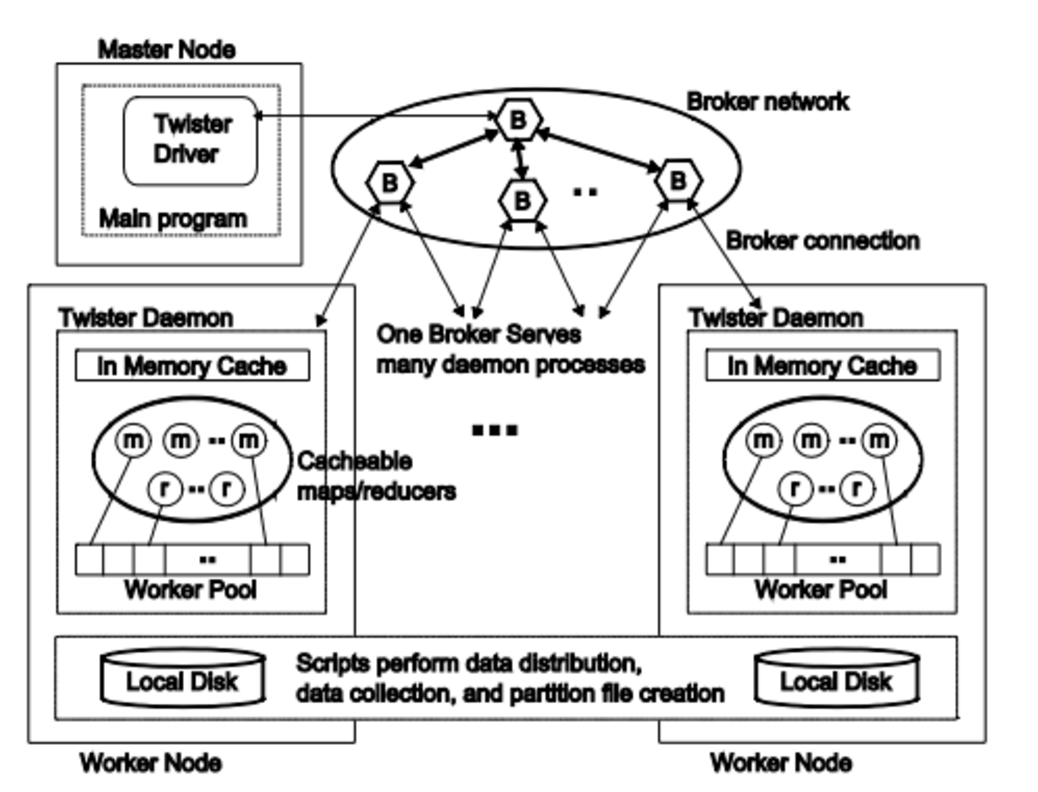
\includegraphics[width=5in]{../figures/twisterarch.pdf}
\caption{Architecture of Twister(摘自\textit{Ekanayake, J.; et al. Twister: a runtime for iterative mapreduce. Proceedings of the 19th ACM International Symposium on High Performance Distributed Computing, 2010})}
\label{fig:twisterarch}
\end{figure}

\subsubsection{Incoop}
Incoop (Incoop: MapReduce for Incremental Computations)同样是一个为了递增计算而修改的MapReduce模型,它不仅仅扩展了MapReduce,还结合了底层分布式文件系统,使得Incoop本身能够检测到输入数据的改变,并且通过一些细粒度的数据重用策略尽量避免不需要的计算,从而提高递增计算的效率。为了达到这个目的,Incoop对Hadoop系统做了几处修改:1)不再使用HDFS来存储输入数据和MapReduce任务的输出数据,Incoop基于一个修改版的Inc-HDFS来存储数据,并且其能够很好的识别出多次循环执行中输入数据中的相似部分;2)为了控制任务的粒度,以尽可能的复用之前的计算结果,Incoop引入了一个新的Contraction阶段;3)Incoop提出了一个基于亲和性的调度算法,以减少task在多次执行过程中数据迁移。
  Inc-HDFS改变了之前HDFS使用的基于固定大小进行分块的做法,转而使用基于内容的方式来进行分块。在Inc-HDFS中,引入了maker的概念,一个maker意味着一个特定的模式。当扫描输入数据进行分块的时候,如果当前所扫描的数据符合某一个maker,那么就将块边界定在此处。当然为了避免过大或者过小的块,其也设置了一些大小限制。
  Incoop中的MapReduce任务执行至少有3个阶段:Map、Contraction、Reduce。所有的map都会将结果持久存储以来,并且把存放的位置信息和map任务的相关信息存放在单独的备忘服务器中,以供日后重复使用。为了减少Reduce任务的粒度,引入了Contraction阶段。Contraction是基于原MapReduce中的combiner实现的。Contraction阶段的结果可以被更好的重用。
  Incoop引入了基于备忘服务器的亲和性调度算法。它试图在尽量提高局部性和减少straggler之间取得平衡。该调度算法为每一个物理节点维护一个单独的任务队列,每一个任务队列都包含了根据备忘服务器的数据而最应该在本节点执行的任务集合。每次取任务都从本节点的任务队列中优先取出,直到为空,方从别的节点“偷取”任务执行。


\subsection{递增处理模型}
\subsubsection{Precolator}
Percolator是由Google于2010年提出的一种事件驱动的处理模型,专用于递增计算。Percolator在Google内部被广泛应用于实时搜索引擎业务,以代替现有基于MapReduce的系统。通过实际使用,Percolator相比MapReduce方案可以提供相同的数据处理量,而将数据处理的更小效率提高了一倍。
  Percolator是专为搜索引擎而设计的。以Google为例,如果爬虫爬取了一部分新的互联网页面,如何处理并且建立索引呢?仅仅因为这一些新数据就重新运行一个MapReduce任务是不合适的,效率太低了。因此递增计算是一个较好的解决方案。Percolator提供了对多达几个PB的数据集的随机访问能力,ACID的事务机制。为了帮助程序员来追踪递增计算的状态,它还提供了观察者机制:一段用来观察指定的数据域改变从而触发执行的代码。一个典型的Percolator程序就是一系列观察者的序列,每一个观察者都可以通过修改数据从而触发下一个观察者。
  Percolator最主要的贡献在于它提供了两个非常重要的实现来支持递增计算:分布式事务以及通知机制。在一个可以随机存取的存储系统之上提供ACID事务是非常困难的,而且该事务是跨行的、跨表的。为了提高效率,Percolator中的事务是通过独立快照实现的,他不能提供串行读写保证,但是却更高效。 Percolator主要是通过Bigtable来实现包括独立快照、读写锁等机制的。锁信息存放在Bigtable的某一列中,为了处理由于节点失效可能导致的死锁,Percolator又引入了主锁的概念。通知机制也是Percolator的一个创新,其中的观察者作为Percolator的基本单元以组成一个应用程序。每一个观察者都会完成一个任务并且通知下一个观察者来执行。该通知机制有点类似于数据库中的触发器,但职责不同。Percolator的观察者实现具有几个优化的地方,首先保证多次触发同一个观察者不会导致任务重复执行;其次提供了一个非常有效的方法来寻找表中改变的项目。
  Percolator在Google的广泛应用,其实表明了基于触发观测和事务机制是可以实现一个高效、可用、可扩放的递增计算模型的。

\subsubsection{Oolong}
\subsection{实时处理模型}
随着Web 2.0站点和移动互联网的兴起,用户开始尝试在互联网上共享更多的数据,而且这些数据的生命期也变得越来越短。对用户提交的新数据进行快速的分析需要能够进行实时计算的编程方法。当然,实时计算的范围相比迭代计算和递增计算可能更宽一点,它有可能包括这两种计算模式中的一部分,然而,实时计算最基本的特点是其对计算时间和计算延迟的关注。

  论文《Analytics for the Real Time Web》中提到了一种扩展已有的Key-Value存储架构以提供实时计算模型的方法。该论文扩展了Cassandra存储系统,加以基于推送的处理协议,增加了对任务执行事务性的特点。总体上来说还是一种基于MapReduce风格的计算模型,不同的是其修改了Reduce函数,变为Reduce*函数。该函数能够递增的接受来数据输入,这也意味着用户可以不断的将数据推送给Reduce*函数,而须一定按照MapReduce框架所规定的那样,只能由Map或者Combiner函数来发送数据。唯一的局限在于并非所有的Reduce函数都可以转化为可以递增计算的Reduce*函数。

\begin{figure}[]
\centering
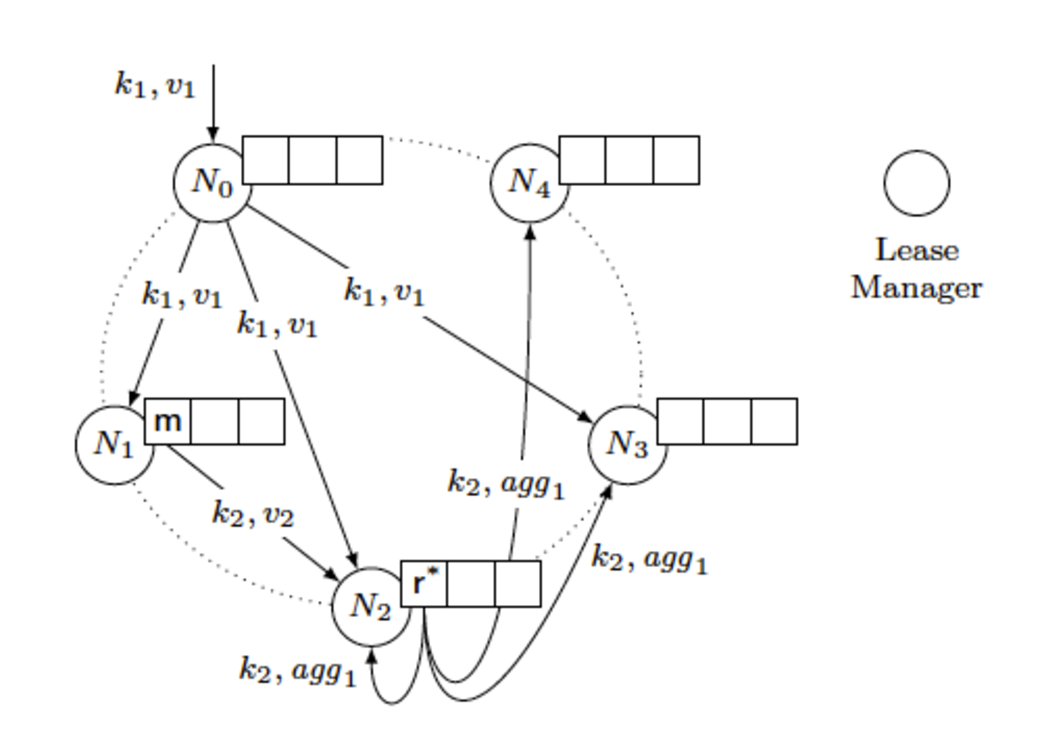
\includegraphics[width=5in]{../figures/realtimep.pdf}
\caption{初始insert以及一个map/reduce*的执行流程(摘自\textit{Analytics for the Real Time Web})}
\label{fig:realtimep}
\end{figure}

  下图展示了一个如何利用本系统进行实时计算的流程。每当一个key-value对被插入到Cassandra系统中的时候,该节点就会执行一个分布式的事务:1)复制该key-value到多个节点;2)选择一个备份节点作为执行map程序的协调者;3)将map任务放入本地的任务队列中。而map任务的执行也是一个分布式的事务:1)将任务从队列中移除;2)将map输出写入到对应的reduce*节点;3)将reduce*任务放入到本地任务队列。而map输出将相同的key值路由到相同的节点中,reduce*的输出会将结果保存到多个节点中。事实上reduce*的执行过程也被视作一个分布式的事务,包括将数据写入多个节点中,以及将reduce*任务正确的从任务队列中移除。

          

Storm也是一个实时计算模型,由2011年由Twitter开放源码使用,Storm主要用于三大类应用:信息流处理,持续计算,分布式远程过程调用。Storm的结构非常类似于Hadoop机群,也是由一个主节点和若干个任务节点组成,不同的是主节点和任务节点之间有一层ZooKeeper机群构成的协调层,用来存放所有的机群状态信息,这样的设计保证了主节点和任务节点都是无状态的,随便杀死主节点或者任务节点都不会影响Storm机群的运行。

\begin{figure}[]
\centering
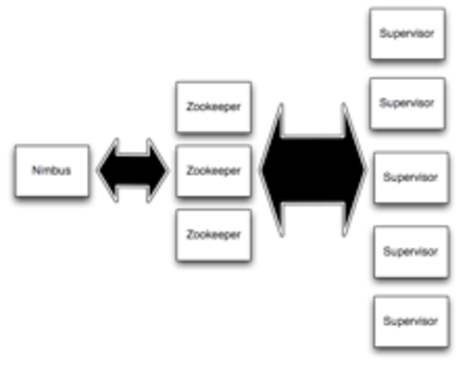
\includegraphics[width=3in]{../figures/storma.pdf}
\caption{Storm系统架构图(摘自\textit{Storm Project Home})}
\label{fig:storma}
\end{figure}

主节点上运行一个叫做Nimbus的守护进行,而任务节点上则运行Supervisor的守护进程。Supervisor监听分配给它的机器,根据Nimbus的委派来启动和关闭工作进行。Storm为了实现流数据分析和持久计算,提供了一个分布式的可靠的方式将流进行转换的标准方式。其中基本组件为“spouts”和“bolts”。一个spouts是一个流的源头,比如一个spouts可以读取元组的一个Kestrel队列并且重发流,或者连接到Twitter的消息流。Bolts用来单步转换流,它基于其输入流创建新的流。其复杂的流转换可能需要用到多个Bolts协同工作。多个步骤的流打包成为一个“topology”(拓扑),提交给Storm执行。如下图所示一个拓扑图:

\begin{figure}[]
\centering
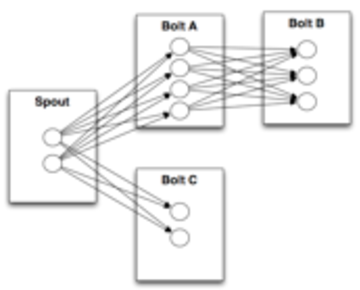
\includegraphics[width=3in]{../figures/stormb.pdf}
\caption{Storm执行流的消息传递(摘自\textit{Storm Project Home})}
\label{fig:stormb}
\end{figure}

任何Storm中的单元都可以以分布式的方式运行。Spouts和Bolts在机群中以多线程的方式运行,并且通过消息机制来传递想要的消息。

\subsection{图模式处理模型}
\subsubsection{GraphLab}

\section{分析}
